\subsubsection{\stid{4.05} STDM07-VeloC: Very Low Overhead Transparent Multilevel Checkpoint/Restart} 


\paragraph{Overview} 

The VeloC project aims to provide a checkpoint/restart framework that
leverages multi-level checkpointing (the combination of several
resilience strategies and heterogeneous storage) to ensure that ECP
applications run to completion with minimal performance overhead. It
delivers a production-ready solution that increases development
productivity by reducing the complexity of having to deal with a
heterogeneous storage stack and multiple vendor APIs. VeloC offers a
client library that can be used directly by the applications or
indirectly by I/O libraries (e.g., HDF5, ADIOS, PnetCDF) to capture
local application states, which are then coordinated and persisted
using a resilience engine. The VeloC software intends to serve ECP
applications such as HACC, NWChem, QMCPACK, LatticeQCD and EXAALT.

\paragraph{Key Challenges}

Applications typically employ simple checkpoint-restart mechanisms to
survive failures that directly use a parallel file system.  However,
I/O bottlenecks to to concurrent writes are a known limitation in this
case. At Exascale, failures are more frequent but the available file
system I/O bandwidth per compute unit decreases. Therefore, there is a
need to checkpoint more frequently but simple checkpointing becomes
even less scalable and efficient. To compensate for the decreasing I/O
bandwidth per compute unit, the storage stack is become increasingly
more heterogeneous (e.g. NVRAM, burst buffers, key-value stores,
etc.). This aspect introduces a new level of complexity for
application developers: they need to adapt their checkpoint strategy
to a variety of new storage sub-systems that may or may not be
available on every machine. This is further amplified by the diversity
of vendors that offer custom APIs. Thus, it is important to provide
a scalable high-performance checkpointing solution that can leverage
the heterogeneous storage stack transparently without sacrificing
ease of use and flexibility.

\paragraph{Solution Strategy}

To address these challenges, VeloC is based on several design principles.

First, it implements multi-level checkpointing. Specifically, it
persists the local checkpoints to other nodes using collaborative
resilience strategies (e.g., partner replication and partner erasure
coding) and to external storage that may include a complex
heterogeneous hierarchy (e.g., parallel file system, burst buffers,
I/O nodes, key-value stores, etc.). Based on experience from previous
efforts such as FTI~\cite{FTI} and SCR~\cite{SCR}, this strategy
greatly improves performance and scalability.

Second, it offers a simple API that enables users to either manually
capture checkpoints into node-local files or to define memory regions
that are automatically serialized into node-local files. All interactions
with the complex heterogeneous storage stack is transparently handled
by VeloC, which facilitates ease-of-use.

Third, VeloC separates the management of node-local checkpoints
from the actual implementation of the resilience strategies by
using a client library that interfaces with a resilience engine.
The engine can be linked directly into the application and will
run in synchronous mode, or it can be part of a separate backend
process that facilitates an asynchronous mode where the resilience
strategies are applied in the background to avoid blocking the
application. This ultimately leads to better performance and scalability.

\paragraph{Recent Progress}

We have interviewed and met with several ECP application team in an
effort to understand their checkpointing needs. Most of our current
efforts involved the HACC, ECP NWChem-X, Lattice QCD and QMCPACK
teams. These interviews helped us understand the needs to the ECP
applications and ensure that they get reflected in the VeloC API
specification. In the last several months, the VeloC team has
developed a stable version of the VeloC API specification, which is
currently in the process of being implemented.

Parallel to the VeloC API definition, we also worked on the
architecture and design of the VeloC software. The VeloC software
design is based on a modular and scalable architecture, as shown in
Figure~\ref{fig:arch}. The design details of the VeloC software
can be found in the VeloC design document, submitted to ECP during
past milestones. Working off the design specification, we implemented
the VeloC software according to the design principles introduced in
the previous section. We have worked on understanding, refactoring,
modularizing several components of the Fault Tolerance Interface
(FTI) and Scalable Checkpoint/Restart (SCR) library to extract
self-contained modules that can be used in the VeloC software. We
recently completed the integration of self-contained modules and
other driver modules into a flexible engine that allows VeloC the
capability of running in synchronous mode directly in the application
processes or in asynchronous mode in a separate active backend
process.

\begin{figure}[t]
\centering
  \begin{subfloat}[Architecture: modular client and engine (running in synchronous and asynchronous mode)\label{fig:arch}]
  	\centering
      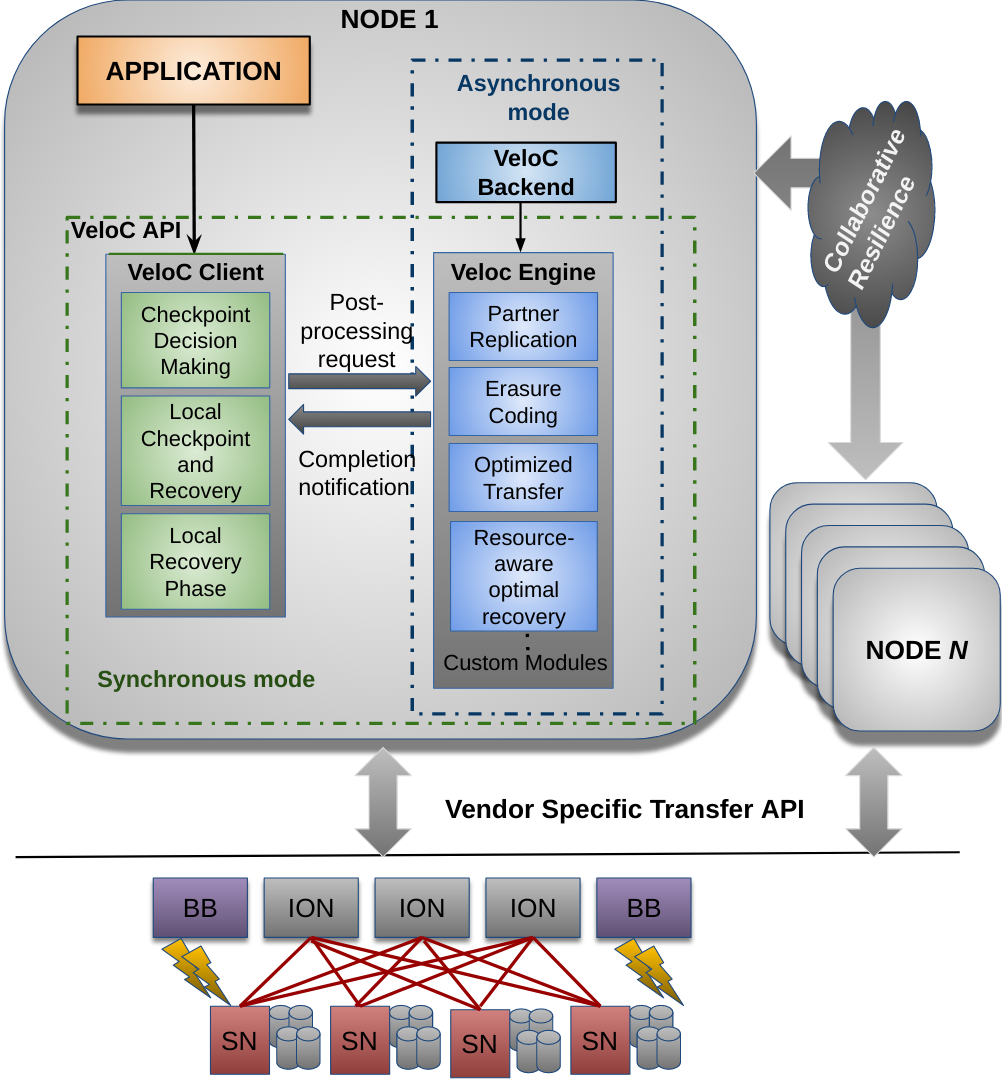
\includegraphics[width=.47\textwidth]{projects/2.3.4-DataViz/2.3.4.05-VeloC/veloc-arch}
\end{subfloat}
  \hfill
  %%
  \begin{subfloat}[Results: checkpointing overhead for a weak scaling experiment (local, local + sync mode, local + async mode). Lower is better\label{fig:res}]
  	\centering
    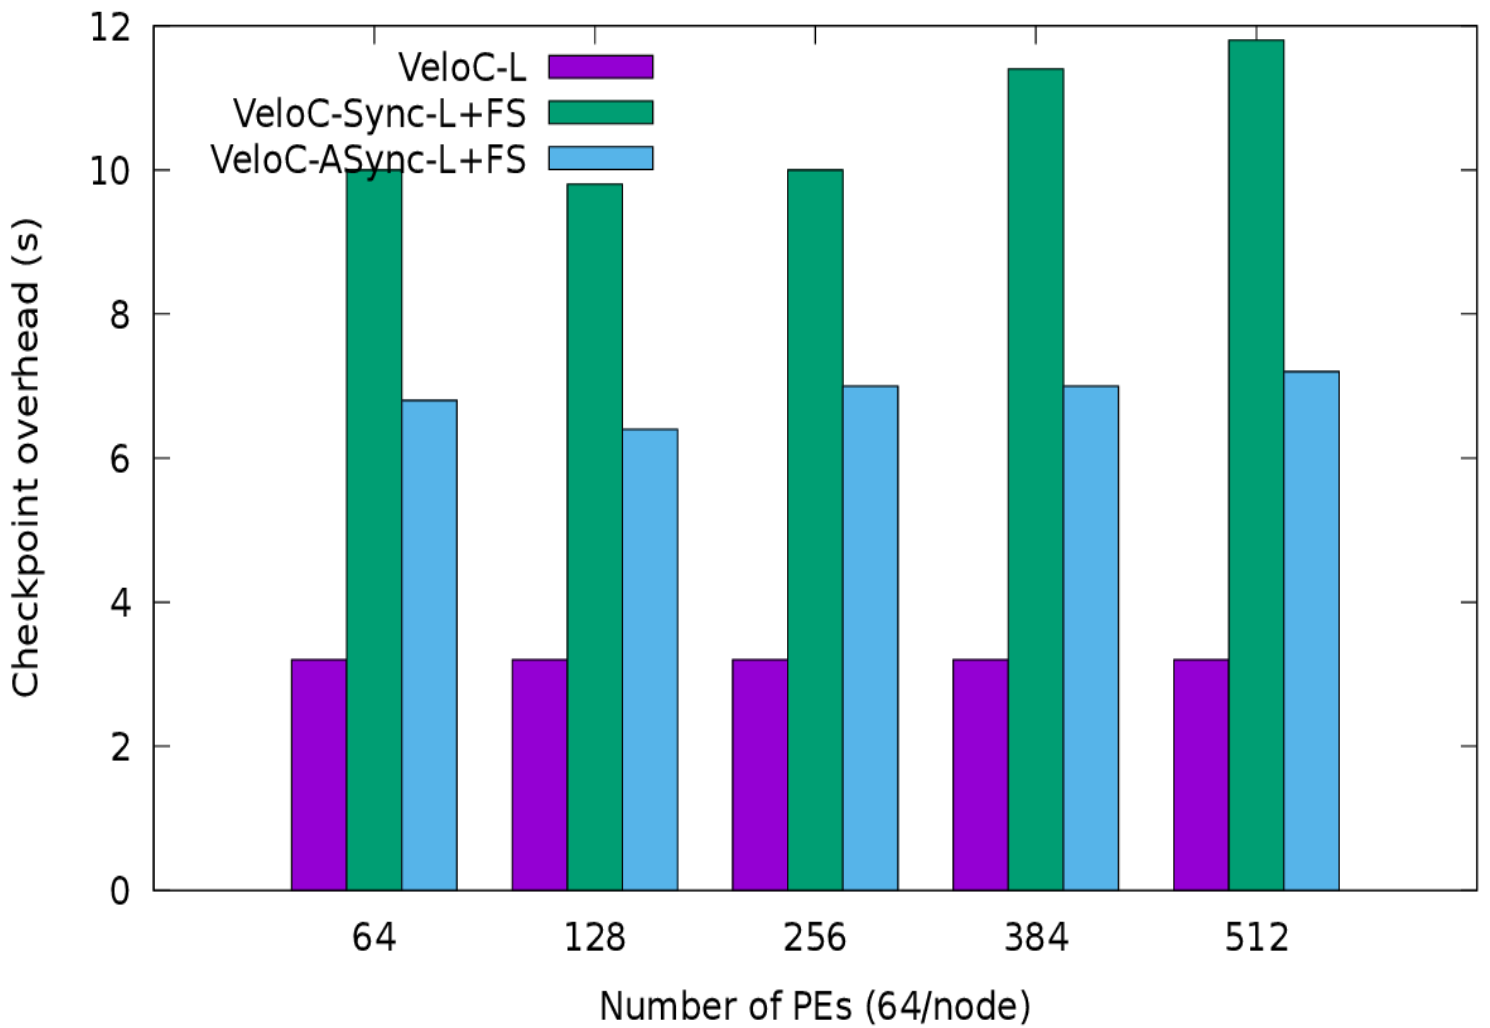
\includegraphics[width=.47\textwidth]{projects/2.3.4-DataViz/2.3.4.05-VeloC/veloc-res}
\end{subfloat}
%  \end{center}
  \caption{VeloC: Very Low Overhead Checkpoint-Restart}%
  \label{fig:veloc}%
\end{figure}


We have run an initial stress test of VeloC on the ANL Theta platform
(KNL nodes, local SSD, Lustre parallel file system) using a heat
distribution application benchmark. The test consists of a weak
scaling experiment (64 processes per node) where the checkpointing
overhead (runtime with a checkpoint vs. baseline without) is measured
for three approaches: (1) node-local checkpoints written to the SSD;
(2) node-local checkpoints followed by synchronous flush to the
parallel file system; (3) node-local checkpoints followed by
asynchronous flush to the parallel file system.  The results are
depicted in Figure~\ref{fig:res}. As can be observed, asynchronous
checkpoints are faster than synchronous checkpoints by a significant
margin and more scalable.

We are also interacting with ALCF to understand the constraints for
VeloC deployment on CORAL systems, such as the configuration of the
resource and job manager and the possibility to run two MPI executions
(application + back-end) on each node.

\paragraph{Next Steps}


The team will be working on the VeloC software release for the next quarter.
Our goal is to finalize the integration and testing of all modules, clean up
the code and run end-to-end testing. Furthermore, we will add documentation
and tutorials to facilitate easy adopting in our user community.
